\chapter{Modelos de iluminaci\'on para tejidos}

Los materiales PBR \textit{MeshStandardMaterial} y \textit{MeshPhysicalMaterial} de ThreeJs, aunque funcionan muy bien para gran parte de
materiales, como pl\'asticos o metales, carecen de par\'ametros que permitan representar los fen\'omenos de retrodispersi\'on o
la reflexi\'on interna caractir\'istica de los tejidos, compuestos de una gran cantidad de hilos que absorben y dispersan la luz.
Es por ello que Filament presenta un nuevo BRDF basado en los trabajos de y que utiliza un par\'ametro de \textit{sheen} para
que ofrece un control sobre el brillo especular para simular los fen\'omenos de reflexi\'on hacia delante y hacia detr\'as
caracter\'istico de tejidos como el terciopelo. Adem\'as algunos materiales absorben parcialmente la luz y la emiten de nuevo,
aport\'ando un color caracter\'istico determinado por las fibras del tejido, \'este fen\'omeno se representa con el par\'ametro
\textit{subsurface} de Filament, que utiliza la aproximaci\'on conocida como \textit{wrapped diffuse lighting} \autocite{orennayar}


\section{Integraci\'on de una nueva clase de material en ThreeJs}
ThreeJs proporciona un API para extender de forma sencilla su librer\'ia de materiales, sin embargo, para proporcionar al nuevo
material de la misma interfaz que los materiales nativos de ThreeJs, as\'i como seguir extendiendo la librer\'ia y ser flexible
a futuros cambios, se ha optado por crear un \textit{fork} de la librer\'ia e introducir los cambios necesarios para crear
este nuevo material. Siguiendo la nomenclatura de ThreeJs: \textit{MeshBasicMaterial}, \textit{MeshStandardMaterial}, etc., el
nuevo material se llama \textit{MeshClothMaterial}.

El nuevo material tiene un BRDF diferente al \textit{MeshPhysicalMaterial},
y diferentes par\'ametros, sin embargo si que soporta los mismos efectos de \textit{normal mapping}, \textit{displacement}, etc.
y comparte gran cantidad de los par\'ametros con el material base, a\~nadiendo \textit{subsurface}, \textit{sheen}.
\textit{MeshClothMaterial} utiliza sus propios \textit{type}, para identificar el tipo
de shader, en la clase \textit{WebGLMaterials} y \textit{defines}, que se utilizar\'an para a\~nadir directivas al c\'odigo GLSL
generado en la clase \textit{WebGLProgram}. Para que el nuevo material est\'e quede expuesto como un material nativo de ThreeJs,
se an\~ade a objeto \textit{Materials}.\\
En la clase \textit{WebGLMaterials} se incluye un nuevo m\'etodo para actualizar los uniforms de \'este nuevo material.

\singlespacing
\begin{lstlisting}[caption=Cambios sobre la clase WebGLMaterials de ThreeJs]
// WebGLMaterials.js

// ...
refreshUniformsCommon( uniforms, material );
// ...
function refreshUniformsCloth( uniforms, material, environment ) {

  refreshUniformsStandard( uniforms, material, environment );

  uniforms.reflectivity.value = material.reflectivity; // also part of uniforms common

  if ( material.sheen ) {

    uniforms.sheen.value.copy( material.sheen );

  } else {

    uniforms.sheen.value.copy( material.color );
    uniforms.sheen.value.r = Math.sqrt( uniforms.sheen.value.r );
    uniforms.sheen.value.g = Math.sqrt( uniforms.sheen.value.g );
    uniforms.sheen.value.b = Math.sqrt( uniforms.sheen.value.b );

  }

  if ( material.subsurface ) {
    uniforms.subsurface.value.copy( material.subsurface );
  }

  if ( material.brdfCloth ) {
    uniforms.brdfCloth.value = material.brdfCloth;
  }
}
// ...
\end{lstlisting}
\singlespacing

\begin{figure}[H]
  \vspace{0.5cm}
  \centering
    \frame{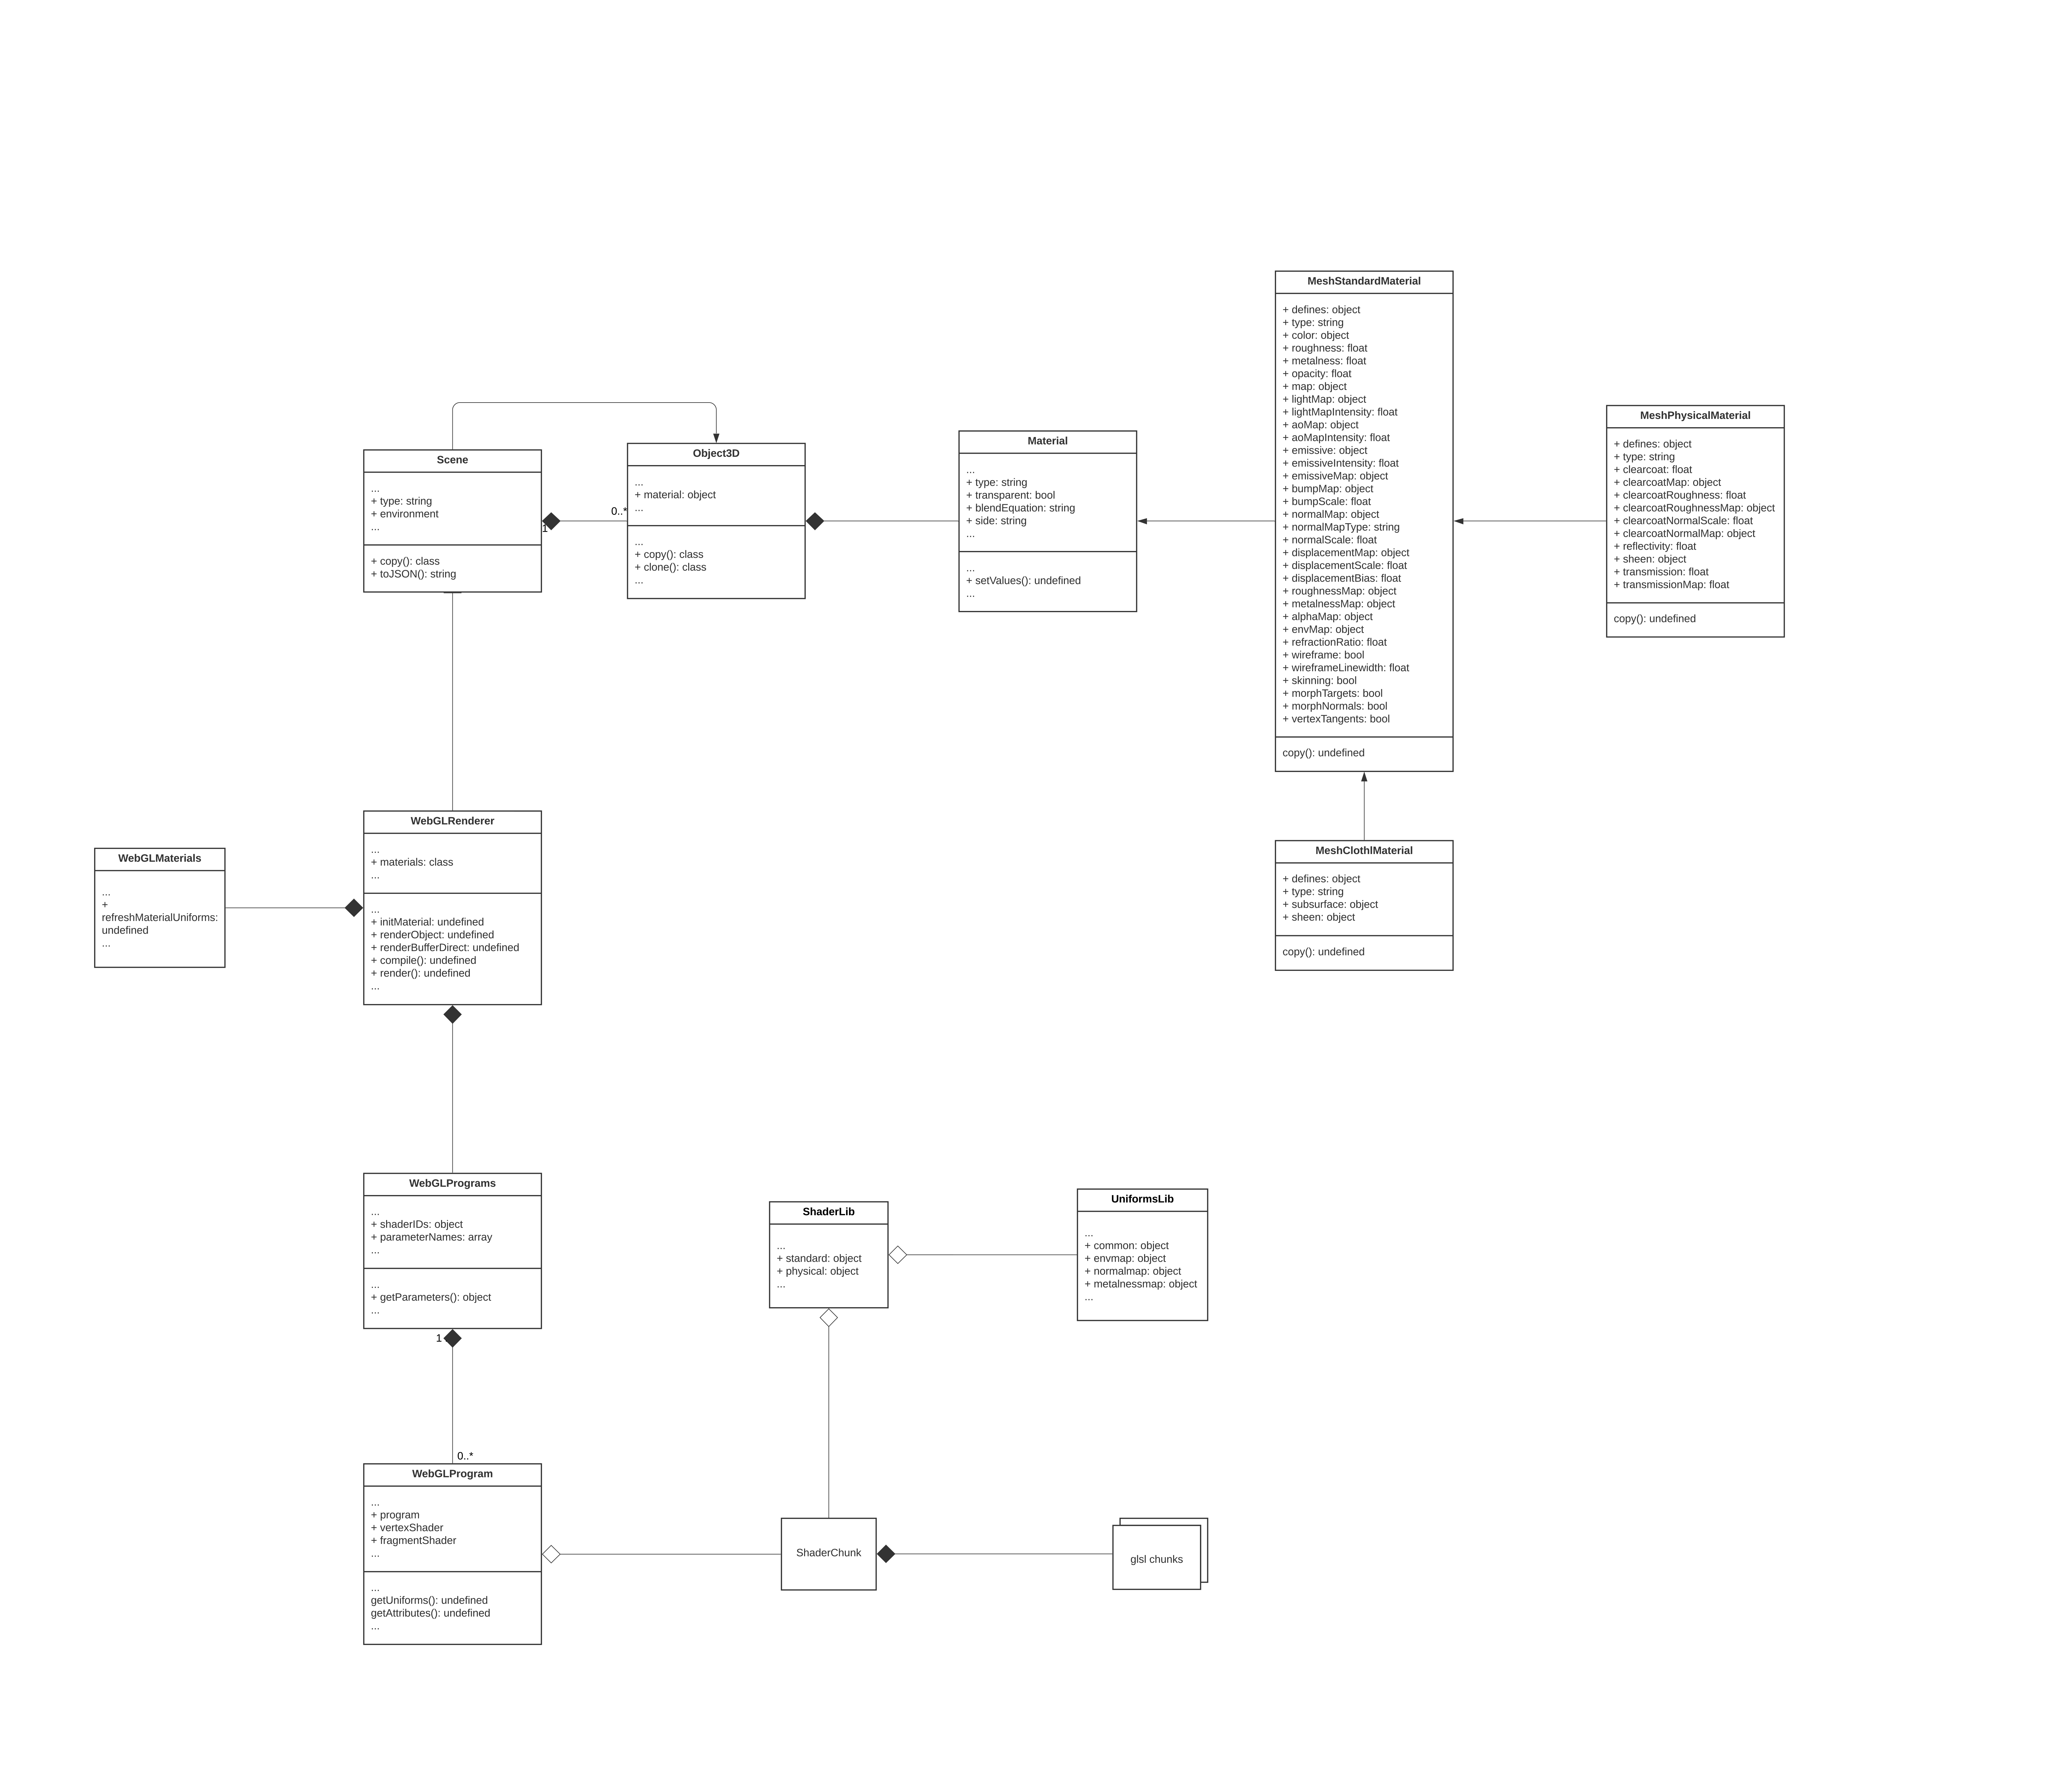
\includegraphics[scale=0.27]{threejs_meshcloth_integration}}
  \caption{Integraci\'on del nuevo material MeshClothMaterial}
\end{figure}
\singlespacing

En la clase \textit{WebGLProgram} se modifica el constructor para para a\~nadir las directivas de precompilaci\'on
para los par\'ametros \textit{subsurface} y \textit{sheen}, en casa de utilizarse estos par\'ametros.\\

\begin{lstlisting}[caption=Cambios sobre la clase WebGLProgram de ThreeJs]
// WebGLProgram.js
// ...
function WebGLProgram( renderer, cacheKey, parameters, bindingStates ) {
  // ...
  prefixFragment = [
    // ...
    ( parameters.sheen || parameters.shaderID === 'cloth' ) ? '#define USE_SHEEN' : '',
    parameters.subsurface ? '#define SUBSURFACE' : '',
    // ...
  ]
  // ...
}
// ...
\end{lstlisting}
\singlespacing

En el closure \textit{WebGLPrograms} se actualiza an\~ade una clave para el nuevo tipo de material, \textit{MeshClothMaterial}
y se a\~nade la cadena de texto \textit{subsurface} al array \textit{parameterNames}, adem\'as de a\~nadir nuevas claves para
el \textit{subsurface} y la informaci\'on precomputada del BRDF, dentro del objeto \textit{parameters} dentro de la funci\'on
\textit{getParameters}. De esta forma nos aseguramos que el sistema interpreta correctamente el nuevo material y puede acceder
y cachear sus propiedades.

\singlespacing
\begin{lstlisting}[caption=Cambios sobre la clase WebGLPrograms de ThreeJs]
// WebGLPrograms.js
// ...
const shaderIDs = {
  // ...
  MeshClothMaterial: 'cloth',
  // ...
};

const parameterNames = [
  // ...
  "subsurface", "brdfCloth",
  // ...
];
// ...
function getParameters( material, lights, shadows, scene, object ) {
  // ...
  const parameters = {
    // ...
    subsurface: !! material.subsurface,
    brdfCloth: !! envMap && shaderID === 'MeshClothMaterial',
    // ...
  };
  // ...
}
// ...
\end{lstlisting}


% ThreeJs utiliza un sistema de chunks (trozos) se componen en tiempo de ejecuci\'on para acabar formando los vertex
% y fragment shaders que se utilizan en los programas de WebGL. Los chunks se componen en la libreria de shaders, la
% clase ShaderLib.
% Para crear nuestro MeshClothMaterial, hemos de extender de la clase base Material, de la que extienden el resto de
% materiales. En este caso, de la misma forma que hace MeshPhysicalMaterial, extenderemos de MeshStandardMaterial,
% que dispone de la mayor parte de uniforms y attributes que necesita nuestro shader.\\

% Para que el motor de render de ThreeJs reconozca este nuevo material es necesario, a\~nadir
% su tipo (MeshClothMaterial) al mapa de ShaderIds para que el gestor de programas (WebGLPrograms)
% lo utilice para detectar obtener los uniforms y shaders necesarios para el material. Adem\'as
% los nuevos par\'ametros necesarios para el material se deben de incluir en el array
% parametersNames, de forma que el sistema de cacheo de programas de ThreeJs detecte estas
% nuevas propiedades.\\

% Finalmente, en el gestor de materiales de ThreeJs, necesitamos a\~nadir un nuevo m\'etodo
% que actualice los unfiroms del programa creado, de la misma forma que se hace con los
% materiales nativos de la librer\'ia.\\

% De esta forma, tenemos un material con la interfaz nativa de ThreeJs, que tiene acceso a los
% chunks definidos en la clase ShaderChunk y cuyos uniforms y composici\'on de chunks definiremos
% en ShaderLib.\\

% El BRDF para el componente especular de la iluminaci\'on directa del material Cloth de Filament,
% se utiliza en ThreeJs para a\~nadir opcionalmente un l\'obulo de Sheen al material. Por otra
% parte, el difuso, utiliza en Filament un t\'ermino opcional para ofrecer una aproximaci\'on
% barata el subsurface scattering para iluminaci\'on directa que utiliza Filament.\\


\vspace{1cm}
\section{Integraci\'on del nuevo \textit{shader} sobre ThreeJs}
  Para a\~nadir un nuevo BRDF hemos de extender el sistema de \textit{chunks} de ThreeJs. Para ello hemos de a\~nadir el
  punto de entrada del nuevo shader al objeto \textit{shaderChunk}. Siguiendo el sistema de nomenclatura de ThreeJs,
  llamaremos \textit{meshcloth\_frag.glsl.js} al nuevo shader, que utiliza chunks comunes con el \textit{MeshStandardMaterial},
  salvo para el c\'aculo de la iluminaci\'on directa e indirecta, que utiliza sus propios \textit{chunks} para el c\'aculo
  de la ecuaci\'on de render: \textit{lights\_cloth\_fragment.glsl.js}, donde se inicializa la estructura de datos relativa
  al material y \textit{lights\_cloth\_pars\_fragment.glsl.js}, donde se calculan las ecuaciones de render de la iluminaci\'on
  directa e indirecta del nuevo material.

  \subsection{Componente difusa}
  El color difuso y el color de \textit{subsurface}, modelan en realidad el mismo fen\'omeno f\'isico, la cantidad de reflexi\'on
  interna que resulta en aportaci\'on sobre la reflexi\'on en direcci\'on al vector de vista. Cuando la distancia de reflexi\'on
  es despreciable en comparaci\'on con el tama\~no del pixel, se aproxima como una reflexi\'on difusa, sin embargo, cuando
  la distancia es considerable, el fen\'omeno se modela de forma diferente. En tiempo real, es com\'un utilizar la citada aproximaci\'on
  \textit{wrapped diffuse lighting} \autocite{orennayar}.
  El modelo para tejidos de Filament utiliza el difuso de Lambert en caso de no utilizar el par\'ametro \textit{subsurface},
  mientras que si lo utiliza utiliza el factor de correci\'on que permite simular los rebotes internos de la luz.

  \begin{equation}
  f_d(v, h) = \frac{c_{diff}}{\pi}
  \Bigg\langle
  n\cdot{l} + \frac{w}{(1+ w)^2}\langle c_{subsurface} + n \cdot{l} \rangle
  \Bigg\rangle
  \end{equation}
  \singlespacing

  \subsection{Componente especular}

  El \textit{MeshPhysicalMaterial} utiliza por defecto un BRDF GGX, \autocite{ggx}. Sin embargo, si el par\'ametro de \text{sheen}
  est\'a activo, utiliza 
  Al contrario que el MeshPhysicalMaterial, que utiliza una una distribucion GGX, el material
  Cloth de Filament utiliza una  version modificada del BRDF presentado por Ashikmin y Premoze
  \autocite{velvet}

  \begin{equation}
  D_{Velvet}(v, h, \alpha) = c_{norm} (
    1 + 4exp \left(\frac{-cot^2\theta_h}{\alpha^2}\right)
  )
  \end{equation}
  \singlespacing

  \hspace{-1.5em}en su lugar se utiliza la la presentada por Est\'evez y Kulla \autocite{sheen}

  \begin{equation}
    D_{Charlie}(\alpha) = \frac
      {(2 + \frac{1}{\alpha})sin(\theta)^\frac{1}{\alpha}}
      {2\pi}
  \end{equation}
  \singlespacing

  \hspace{-1.5em}y se utiliza una version modificada del denominador para suavizar el degradado de la sombra.

  \begin{equation}
  \frac{1}{4(n\cdot{l} + n\cdot{v} - (n\cdot{l})(n\cdot{v}) )}
  \end{equation}
  \singlespacing

  \subsection{Iluminaci\'on indirecta}
    ThreeJs utiliza dos enfoques, por una parte, mapas de irradiancia y por otra, light probes, que
    utilizan spherical harmonics. Los mapas de irradiancia son una tecnica IBL (Image Based Lighting)
    tratan todo el entorno como una fuente de luz y utilizan im\'agenes precomputadas que permiten
    acelerar este calculo. Estas t\'ecnicas, aunque muy eficientes durante la ejecucion, son muy
    costosas como para generarlas en tiempo real bajo demanda, la tecnica spherical harmonics, una
    t\'ecnica que reduce el coste de generacion de los mapas de entorno a costa de comprimir la
    informacion de irradiancia en un representacion frecuencias frente a espacio.

    \subsubsection{Componente difusa}
      La parte integral de la ecuaci\'on se resuelve utilizando el mapa de irradiancia,
      que utiliza un factor de correci\'on en caso de estar modelando la refracci\'on interna,

      $$
      L_o(p, w_o) = k_d \frac{c}{\pi} \int_{\Omega}{L_i(p, w_i) n\cdot{w_i}dw_i}{}
      $$

      \begin{lstlisting}
float diffuseWrapFactor = 1.0;
#if defined(SUBSURFACE)
  diffuseWrapFactor *= saturate((dotNV + 0.5) / 2.25);
#endif

// Combine envmap and SH diffuse irradiance
vec3 Fd_SH = reflectedLight.indirectDiffuse * ( 1.0 - E ) * diffuseWrapFactor;
vec3 Fd_Lod = irradiance * BRDF_Diffuse_Lambert( material.diffuseColor )  * ( 1.0 - E ) * diffuseWrapFactor;
vec3 Fd = Fd_SH + Fd_Lod;

#if defined(SUBSURFACE)

  Fd *= saturate(subsurface + dotNV);

#endif
      \end{lstlisting}
      \singlespacing

    \subsubsection{Componente especular}
    \bgroup
      Para el especular, la tanto ThreeJs utilizan la t\'ecnica split-sum approximation
      \autocite{unreal}. \'Esta t\'ecnica permite separar la en dos partes la soluci\'on de la
      integral.

      \begin{equation}
        \resizebox{0.95\hsize}{!}{%
        $L_o(p, w_o) =
        \int_{\Omega} k_s \frac{DFG}{4(w_o\cdot{n})(w_i\cdot{n})})L_i(p, w_i)n\cdot{w_i}dw_i = \\
        \int_{\Omega} k_s \frac{DFG}{4(w_o\cdot{n})(w_i\cdot{n})}) *
        \int_{\Omega}L_i(p, w_i)n\cdot{w_i}dw_i$   
        }
      \end{equation}
      \singlespacing

      Por una parte, el mapa prefiltrado de entorno es un mapa preconvolucionado que tiene en cuenta
      los posibles valores de rugosidad del material de forma que a medida que el ruido es mayor, las
      reflexiones son de un color menos definido. Esta tecnica utiliza simplifica el calculo de
      la integral asumiendo la direccion de la vista igual a la direccion de sampleo.\\
      Por otra parte, el c\'alculo del BRDF se almacena en una textura, conocida como mapa de integral
      del BRDF, utilizando $n\cdot{w_i}$ en el eje $x$ y $roughness$ en el eje y.

      \begin{figure}[H]
        \vspace{0.5cm}
        \centering
          \frame{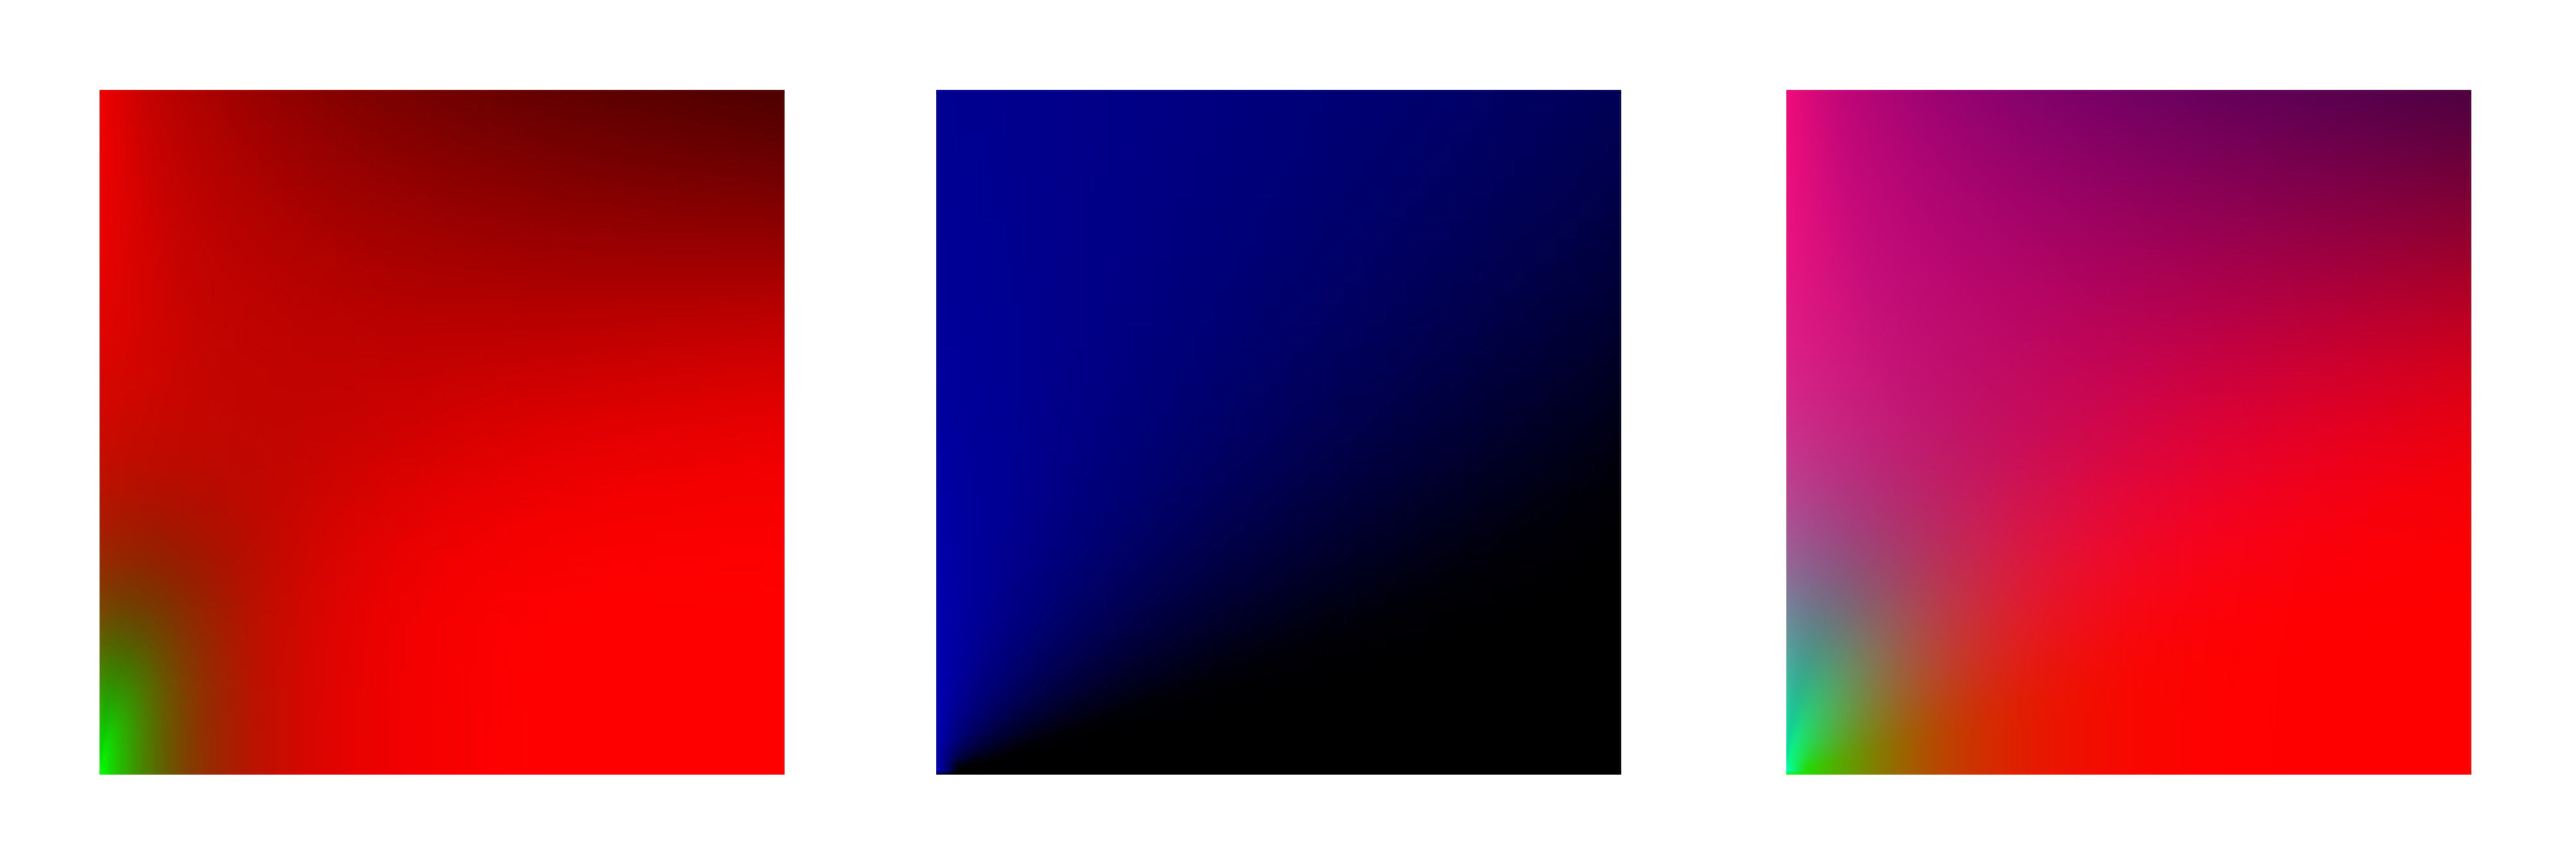
\includegraphics[scale=0.4]{splitsumcloth}}
        \caption{DFG tela}
      \end{figure}

      ThreeJs utiliza la aproximaci\'on anal\'itica para el c\'alculo de de mapa de integral del BRDF,
      la presentada por Epic Garmes \autocite{shadingmobile}, para aproximar el c\'alculo el BRDF GGX.\\

      \begin{lstlisting}[caption=Apromixaci\'on anal\'itica a la integral del BRDF en ThreeJs]
      vec2 integrateSpecularBRDF( const in float dotNV, const in float roughness ) {
        const vec4 c0 = vec4( - 1, - 0.0275, - 0.572, 0.022 );
        const vec4 c1 = vec4( 1, 0.0425, 1.04, - 0.04 );
        vec4 r = roughness * c0 + c1;
        float a004 = min( r.x * r.x, exp2( - 9.28 * dotNV ) ) * r.x + r.y;
        return vec2( -1.04, 1.04 ) * a004 + r.zw;
      }
      \end{lstlisting}
      \singlespacing

      Sin embargo, \'este c\'aculo no es v\'alido para nuestro BRDF, por que, deberemos utilizar una
      tabla en la que almacenar los resultados calculados para el BRDF presentado por Est\'evez y Kulla.
    \egroup

\vspace{1cm}
\section{Resultados}

A continuaci\'on se muestran y comentan las im\'agenes como resultado de la implementaci\'on. Los resultados se centran
en el an\'alisis de las citadas propiedades \textit{sheen} y \textit{subsurface} del material \textit{MeshClothMaterial}.
% Por una parte se muestran interpolaciones de dichas propiedades frente a un color base constante y por otra,

\begin{figure}[H]
  \vspace{0.5cm}
  \centering
    \frame{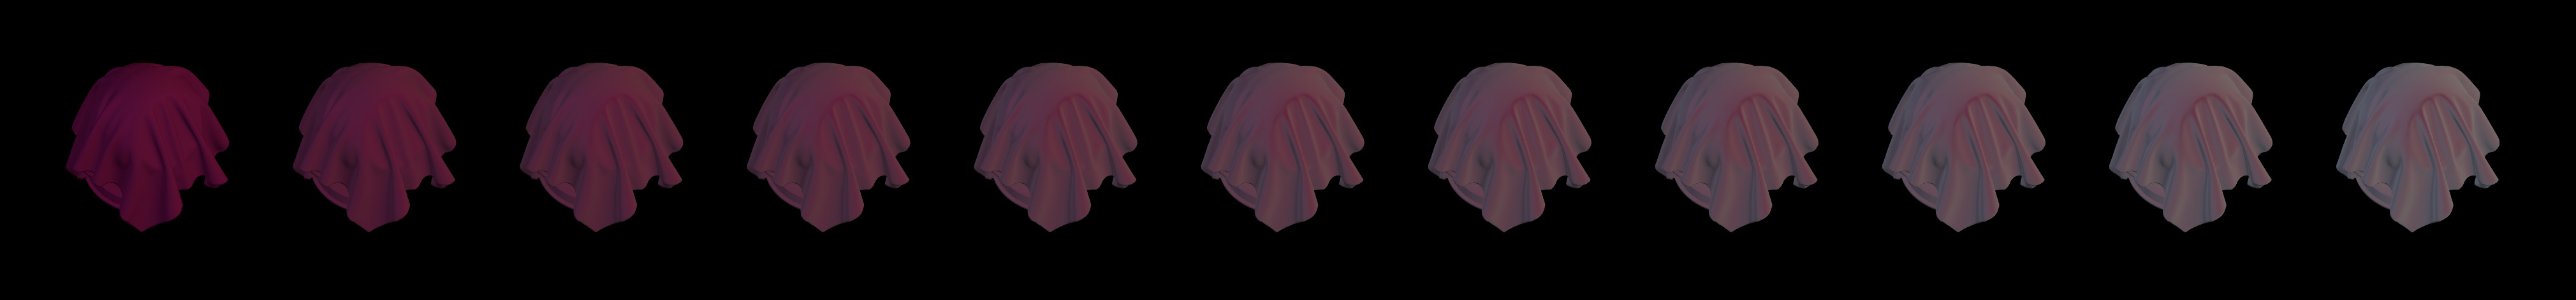
\includegraphics[scale=0.2]{results/sheenintensity.jpg}}
  \caption{Interpolaci\'on de un color de \textit{sheen} aumentando su luminosidad frente a un color base constante.}
\end{figure}

El nuevo material no ofrece un control directo sobre la intensidad del \textit{sheen}, sin embargo, un efecto similar se puede
alcanzar utilizando un el mismo que el color base aumentando la luminosidad. De \'esta forma se consigue que el l\'obulo
de \textit{sheen} produzca reflexiones m\'as brillantes (figura 6.3).

\begin{figure}[H]
  \vspace{0.5cm}
  \centering
    \frame{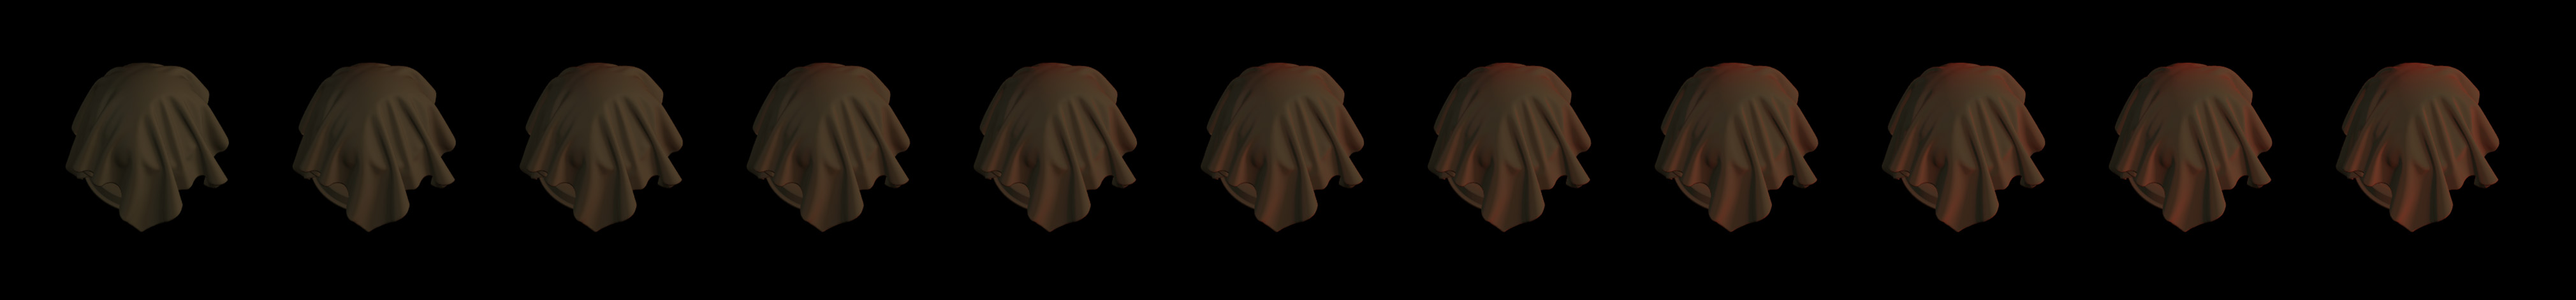
\includegraphics[scale=0.2]{results/sheentint.jpg}}
  \caption{Interpolaci\'on de un color de \textit{sheen} aumentando su saturacion frente a un color base constante.}
\end{figure}
\singlespacing

Como se muestra en la figura 6.4, utilizar un color de \textit{sheen} diferente al color base permite conseguir reflexiones especular en dos tonos como
resultado de la combinaci\'on del l\'obulo primario y el l\'obulo de sheen.

\begin{figure}[H]
  \vspace{0.5cm}
  \centering
    \frame{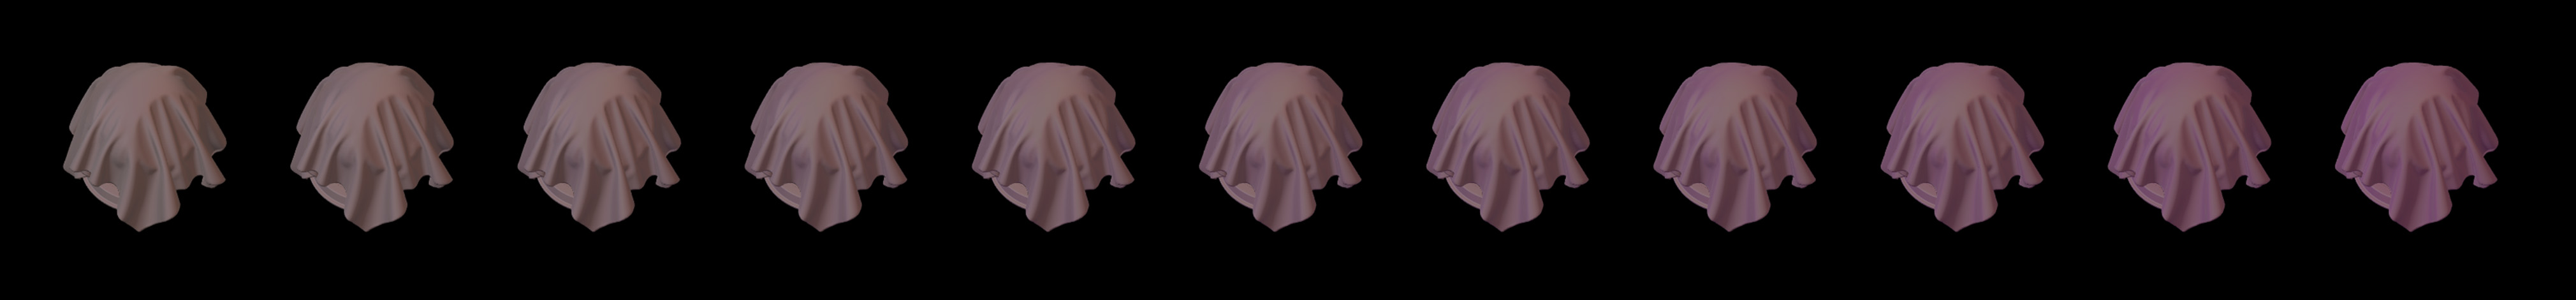
\includegraphics[scale=0.2]{results/subsurfaceintensity.jpg}}
    \caption{Interpolaci\'on de un color de \textit{subsurface} aumentando su saturaci\'on frente a un color base constante.}
\end{figure}
\singlespacing

En la figura 6.5, el color base permanece constante, mientras que el \textit{subsurface}, de un tono similar al color base,
aumenta su saturaci\'on. Del mismo modo que en el \textit{sheen}, jugando con el valor de luminosidad del \textit{subsurface},
se puede obtener control sobre la intensidad del efecto.


\begin{figure}[H]
  \vspace{0.5cm}
  \centering
    \frame{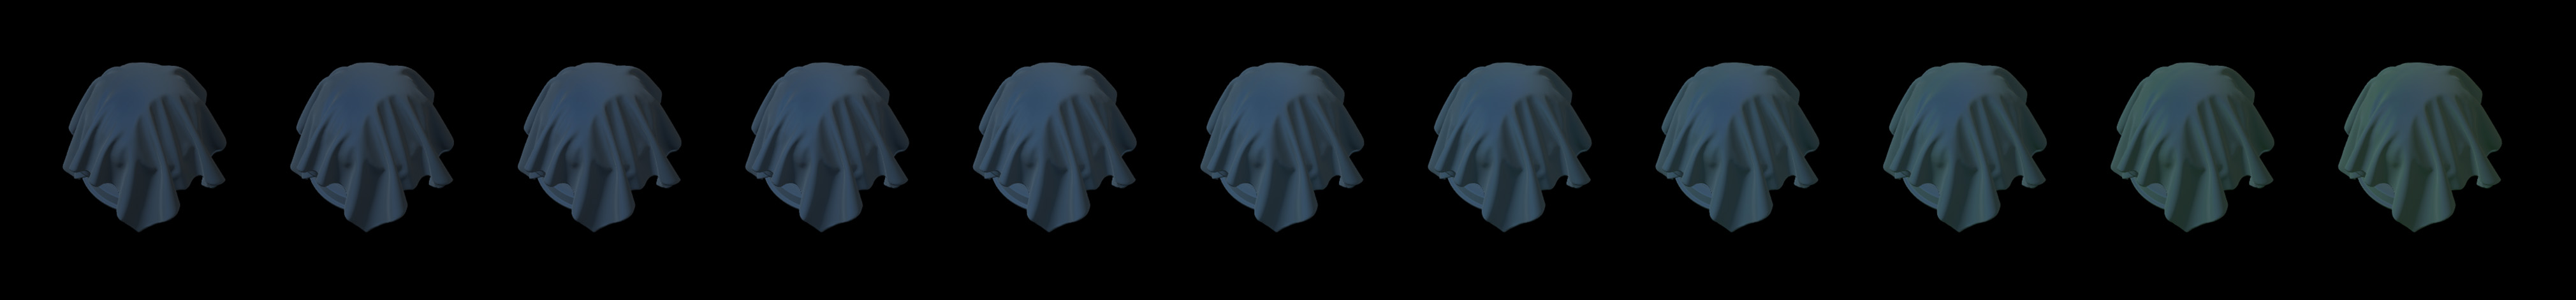
\includegraphics[scale=0.2]{results/subsurfacetint.jpg}}
    \caption{Interpolaci\'on de un color de \textit{subsurface} aumentando su luminosidad frente a un color base constante.}
 \end{figure}
\singlespacing

En la figura 6.6, se utilizan dos tonos de color complementarios para el color base y el \textit{subsurface}. El color
base es constante, mientras que el \textit{sheen} aumenta por pasos su saturaci\'on.
El factor de correcci\'on aplicado sobre el color difuso, que simula el efecto de reflexi\'on interna, ti\~ne progresivasivamente
las sombras del color asignado al par\'ametro \textit{subsurface}.\\

Las siguientes comparativas son matrices bidimensionales que muestran la evoluci\'on de un par\'ametro por cada uno de los ejes
$x$ e $y$ y permiten ver la relaci\'on entre estos dos par\'ametros y su efecto sobre la apariencia final del material.\\

En la comparativa de la figura 6.7, se muestra en el eje $x$ un aumento del efecto de \textit{sheen}, mientras que en el
eje $y$ aumenta el valor de roughness del material. Se puede apreciar que con valores bajos de \textit{sheen}, el efecto
se aprecia con intensidad en los \'angulos cr\'iticos y decae r\'apidamente, mientras que para valores altos de este par\'ametro,
el efecto se extiende hacia los tonos medios, creando una transici\'on m\'as suave entre el color base y el de \textit{sheen}.\\

La figura 6.8 muestra los incrementos del color de \textit{sheen} en el eje $x$ e incrementos en el eje $y$ del color de subsurface.
El \textit{sheen} de color verde simula el efecto de retrodispersi\'on que ti\~ne el brillo especular de \'este color, mientras
que el \textit{subsurface}, de color rojo, da a los tonos medios un color rojizo. El valor de \textit{roughness} del material
es alto, es por ello que a medida que aumentan los valores de \textit{subsuface}, \textit{sheen}, se aprecia una transici\'on
suave entre estos dos par\'ametros, que proporcionan el aspecto amarillo/anaranjado, como resultado de la transici\'on entre
el verde del brillo especular y el rojo de las sombras y tonos medios.

\begin{figure}[H]
  \vspace{0.5cm}
  \centering
    \frame{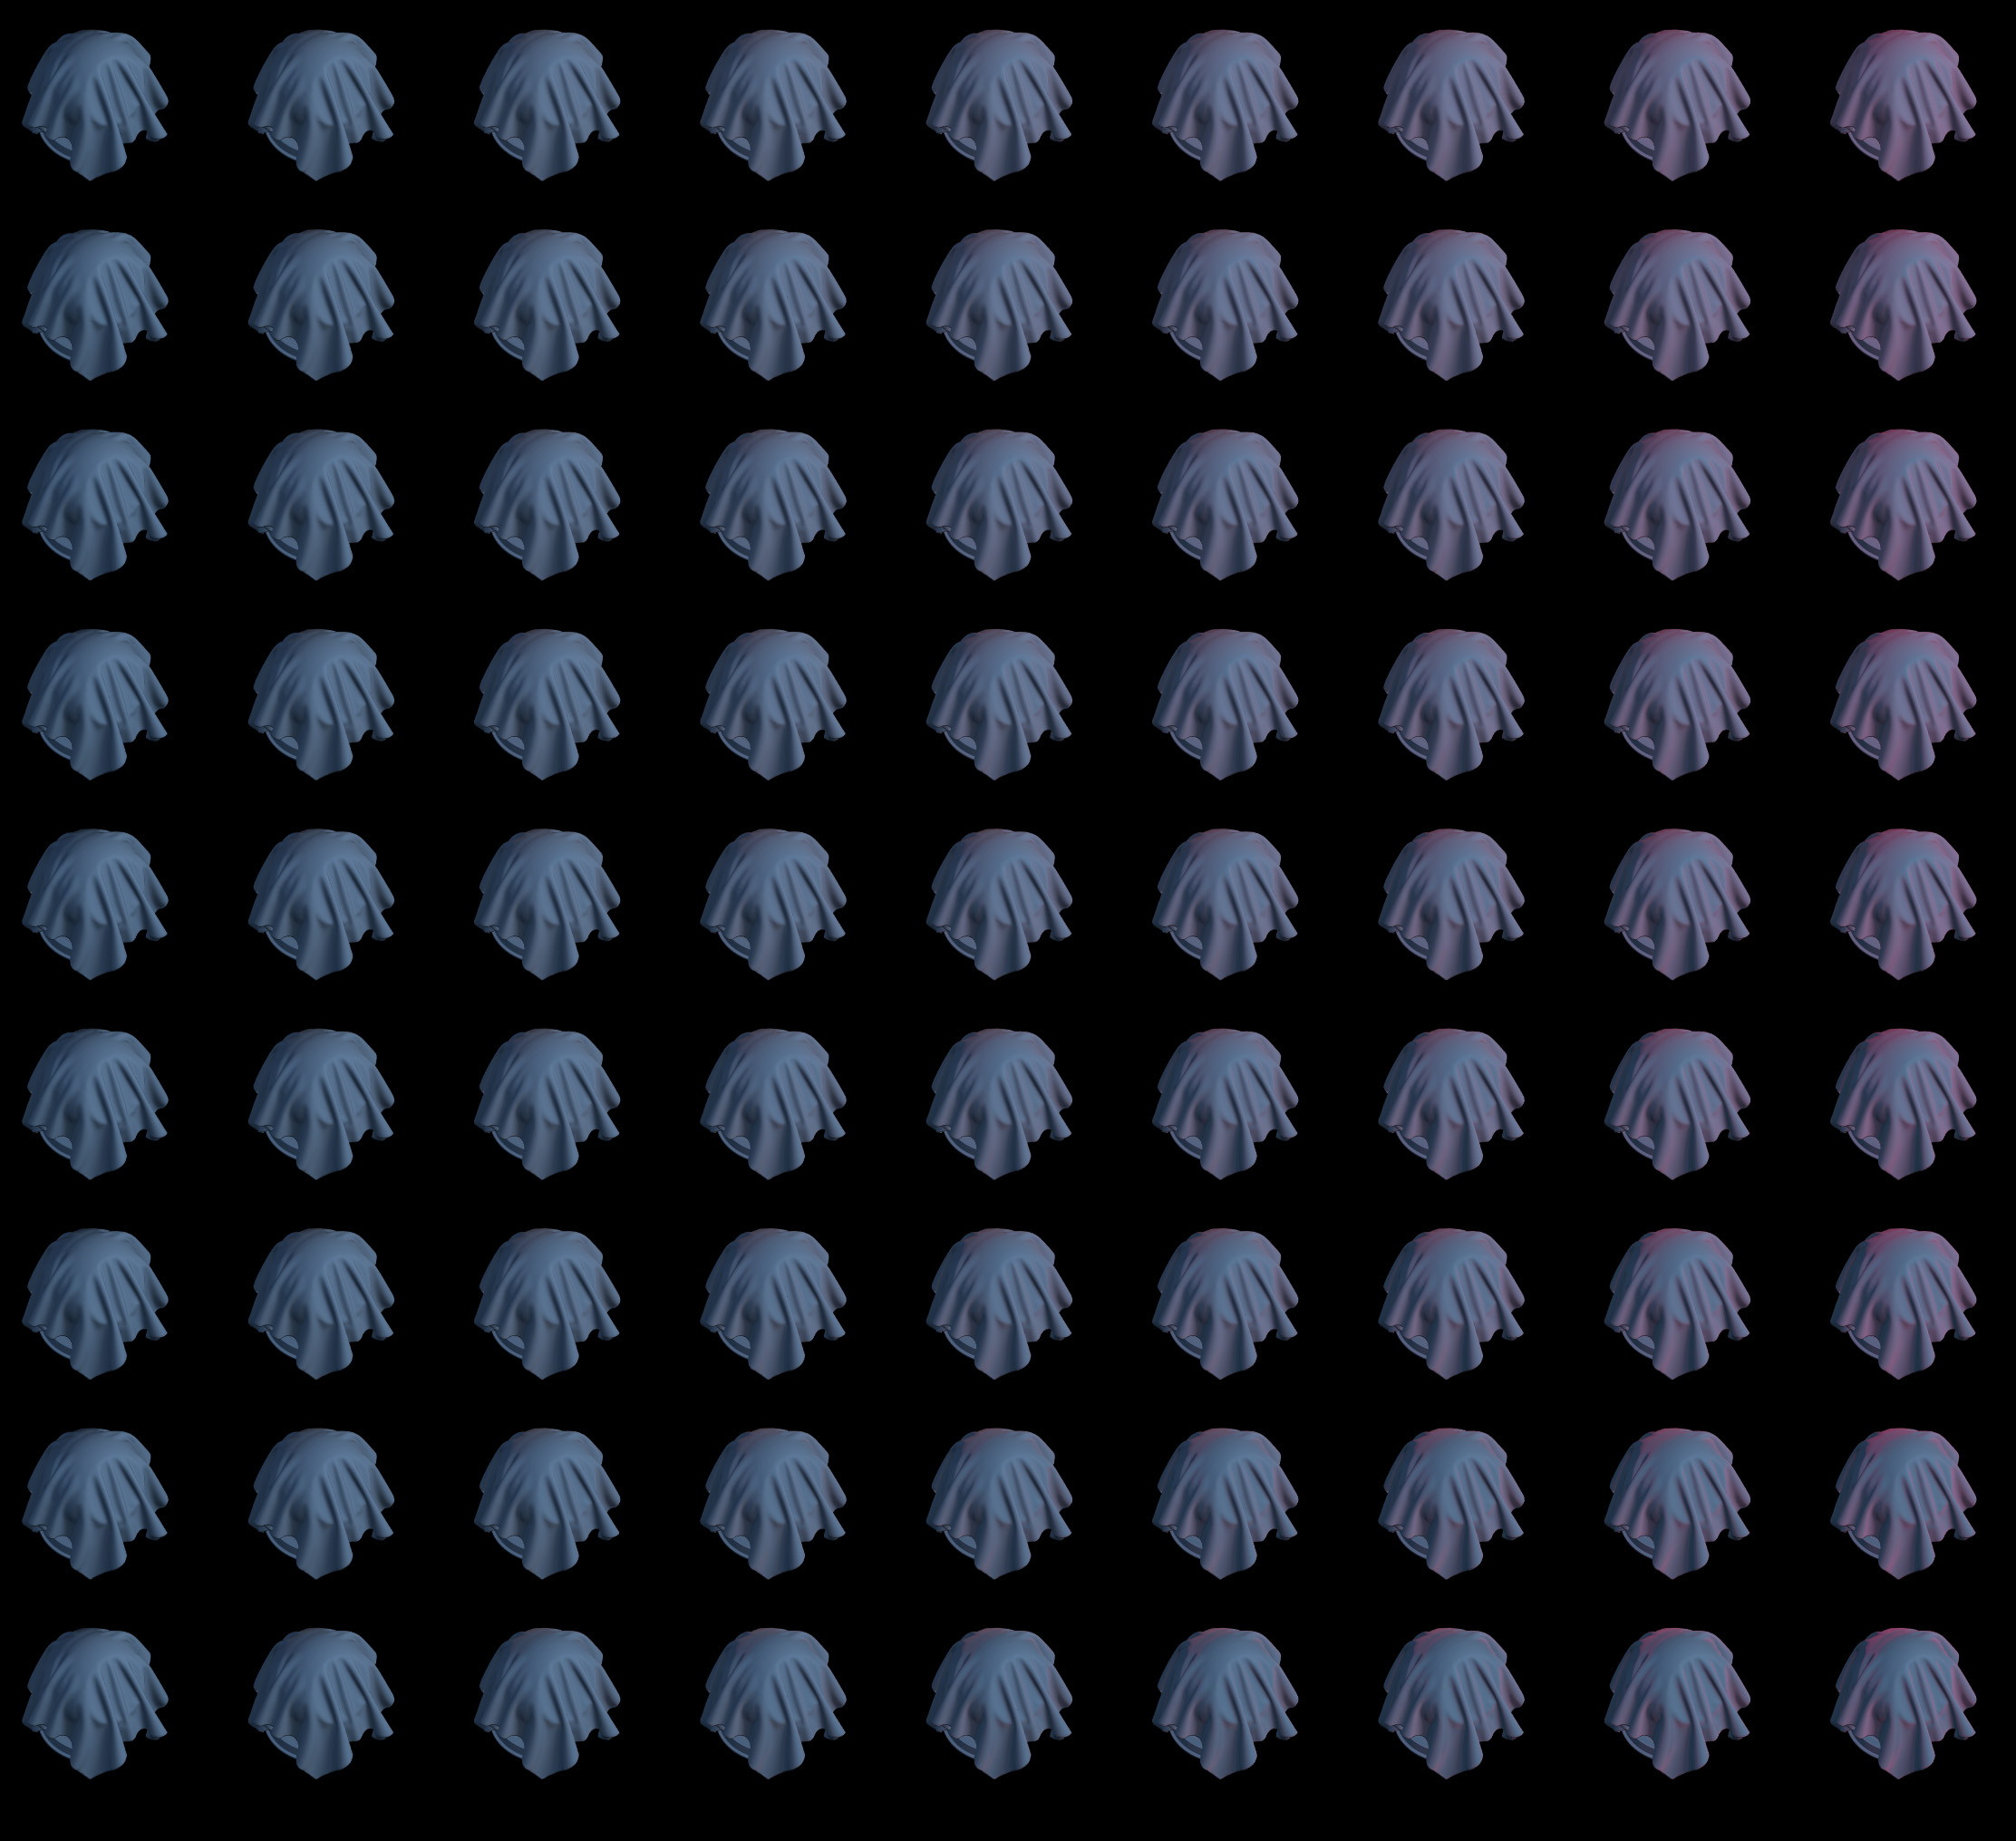
\includegraphics[scale=0.37]{results/grid_sheen_roughness.jpg}}
    \caption{En el eje $x$ aumenta la intensidad del \textit{sheen}, en el eje $y$ el valor de \textit{roughness}.}
  \vspace{0.5cm}
\end{figure}
\singlespacing

\begin{figure}[H]
  \vspace{0.5cm}
  \centering
    \frame{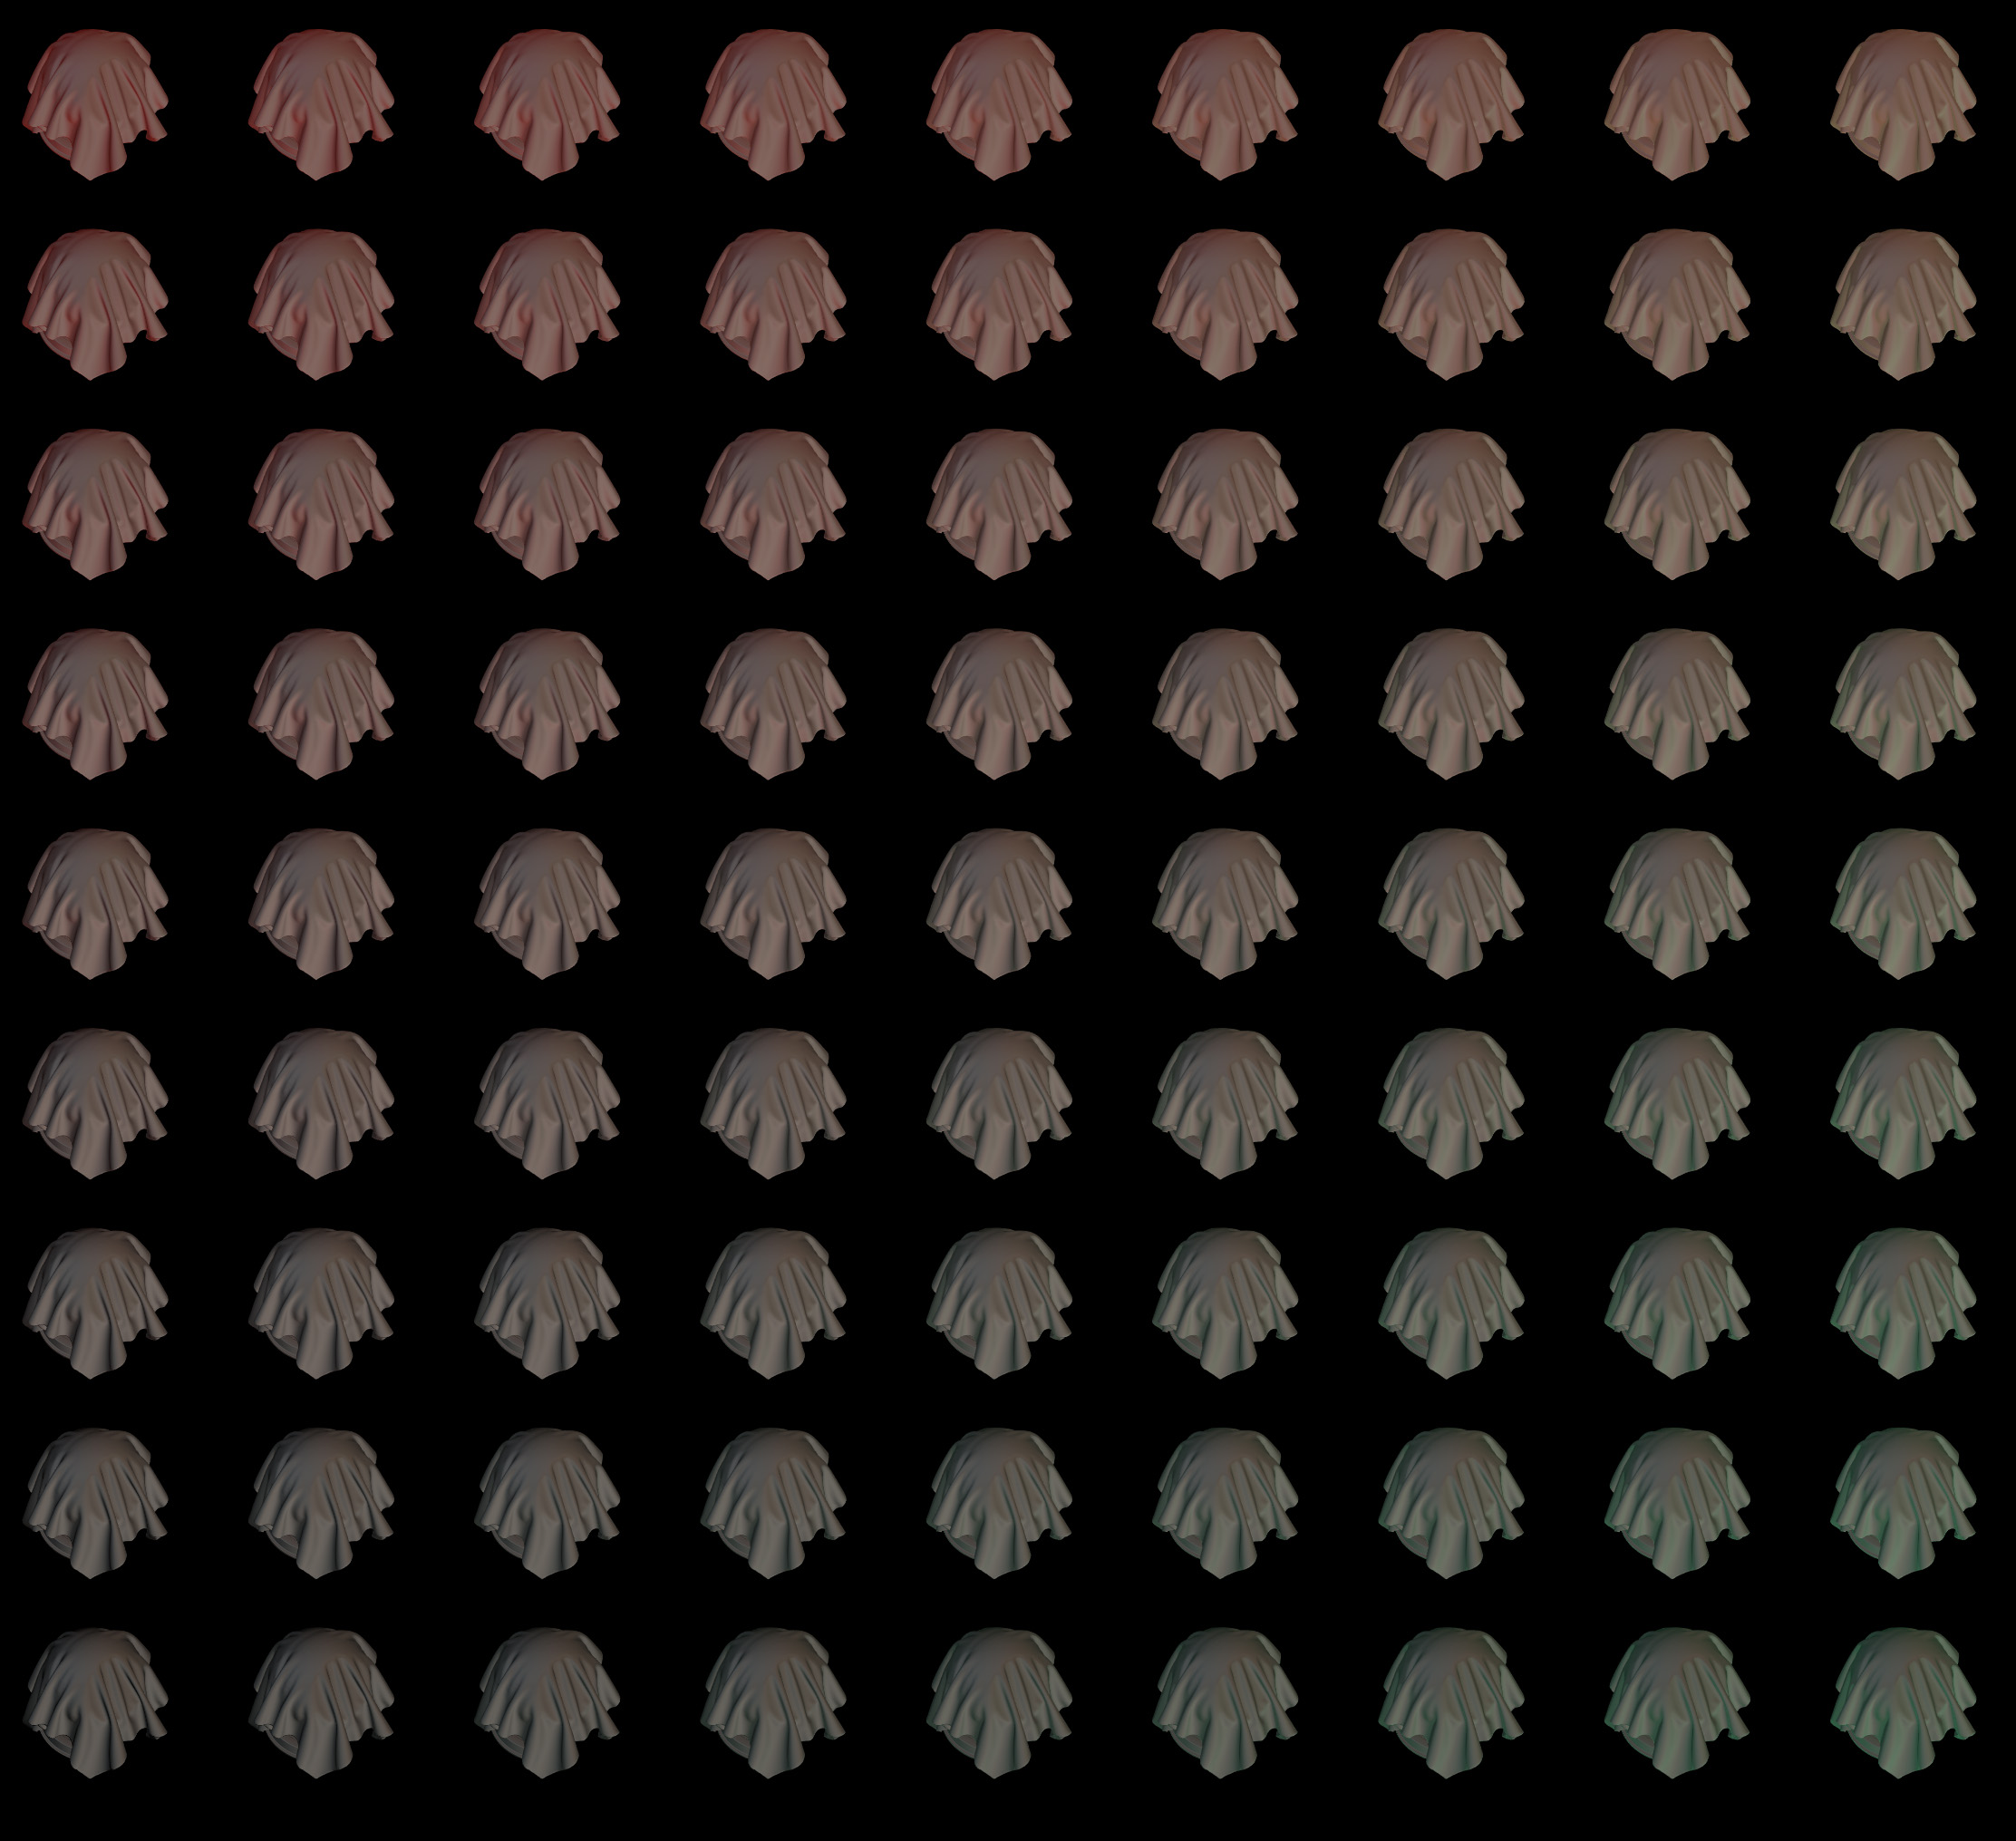
\includegraphics[scale=0.37]{results/grid_sheen_subsurface.jpg}}
  \caption{Integraci\'on del nuevo material MeshClothMaterial}
  \vspace{0.5cm}
\end{figure}
\singlespacing